\section{Phương pháp đề xuất}

\subsection{Adaptive Graph Convolution Network}
Hình \ref{fig:agcn} được nhóm trích từ bài báo \cite{shi2020skeleton} biểu diễn mô hình AGCN mà nhóm lấy ý tưởng.


Dữ liệu đầu vào của layer AGCN gồm ma trận có kích thức $C_{in} \times T \times N$. Trong đó $C_{in}$ là số chiều của tọa độ biểu diễn khớp (trong tập dữ liệu nhóm lựa chọn thì $C_{in} = 3$ tương ứng với tọa x,y,z trong không gian 3 chiều), $T$ là số frame hình và $N$ là số khớp của khung xương (trong tập dữ liệu nhóm chọn có 25 khớp).

Ban đầu dữ liệu liệu sẽ được đi qua 2 mạng tích chập với kích kernel là $1 \times 1$ để nhúng tọa độ $C_{in}$ chiều thành 1 vector nhúng có kích thước $C_e$ mang nhiều kích thức hơn vector tọa độ ban đầu ($C_e > C_{in}$). Từ đây ta nhân 2 ma trận sau khi nhúng để được ma trận kích thước $NxN$, và cho qua hàm softmax theo cột ta được ma trận $C_k$. Khi đó mỗi cột có thứ tự $i$ của ma trận $C_k$ là một phân phối xác xuất có $N$ phần phần tử , với mỗi phần thử thể hiện mới độ tương quan của các đỉnh đối với khớp $i$. Từ đây $C_k$ chính là trọng số để số xây dựng adaptive matrix (AM).

$B_k$ chính là ma trận liền kề được xây dựng từ dữ liệu skeleton ban đầu gồm các cạnh được nối một cách tự nhiên theo khung xương con người. Một ma trận liền kề mới là $C_k + B_k$ mang thêm các cạnh mà mô hình cho là quan trọng trong việc phân loại hành động.

Ma trận trận liền kề mới sẽ được nhân vào dữ liệu ban đầu để thay đổ lại mức độ quan trọng giữa các đỉnh. Sau đó tiếp tự được đưa qua lớp tích chập có kernel $1 \times 1$ để nhúng vector tọa độ ra kích thước $C_{out}$ mà nhóm mong muốn nhằm trích suất nhiều thông tin hơn từ một khớp.

Khác với tập RGB, các mô hình học máy thường nhúng một vùng ảnh RGB qua tích chập thì ở dữ liệu skeleton ta nên nhúng từng khớp. Bởi một pixel trong ảnh RGB mang rất ít kiến thức, nhưng một khớp có tọa độ x, y, z lại chứa rất nhiều kiến thức.

Hình \ref{fig:morebones} cho thấy kết quả sau khi đi qua các layer AGCN, cạnh màu xanh là cách cạnh của khung xương người ban đầu, màu cam là các cạnh được mô hình học và nối thêm.

\begin{figure}[!ht]
    \begin{center}
        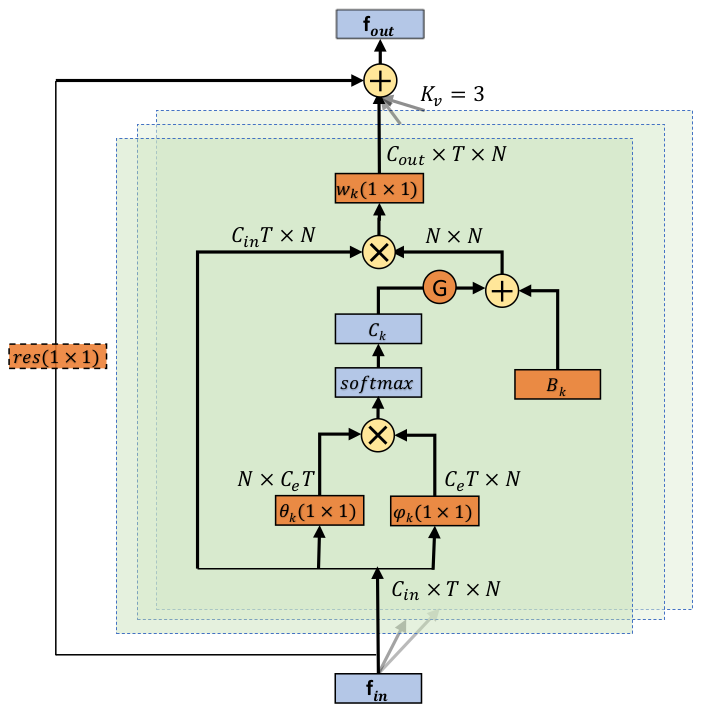
\includegraphics[width=\linewidth]{asset/image/agcn.png}
        \caption{Adaptive graph convolutional network}
        \label{fig:agcn}
    \end{center}
\end{figure}

Mô hình này đã được nhóm hiện thực lại bằng Pytorch và trình bày ở mục \ref{section:result}

\subsection{Hướng đề xuất cải tiến mô hình}

Ngoài ý tưởng về AGCN, nhóm đã tìm đọc thêm nhiều tài liệu để lựa chọn hướng đi mới nhằm kết hợp lại và tăng cường độ chính xác mô hình:

\begin{itemize}
    \item Ở bước tiền xử lý nhóm quyết định sẽ tăng cường dữ liệu theo 2 hướng nhằm tăng kiến thức về không gian và thời gian. Về mặt thời gian, nhóm sẽ hiệu tọa độ của các khớp tương ứng giữa các frame hình liền kề nhau nhằm tạo ra kiến thức về chuyển động. Về mặt không gian, nhóm hiệu tọa độ các đỉnh liền kề nhau theo cấu trúc khung xương con người nhằm tạo ra kiến thức khúc xương. Đầu vào của mô hình sẽ bao gồm 3 luồng, là dữ liệu gốc, dữ liệu tăng cường theo thời gian và dữ liệu tăng cường theo không gian.
    \item Ở mô hình baseline nhóm lựa chọn, bottleneck xảy ra ở lớp fully connected, số tham số quá lớn để có thể phân loại dữ liệu với 25 khớp xương, 300 frame hình, là số chiều của vector nhúng được tăng cường lên tới 32 chiều. Vì vậy nhóm tìm hiểu và lấy ý tưởng từ bài báo \cite{song2020stronger} nhằm nhúng 5 bộ phận cơ thể của con người là đầu, 2 tay và 2 chân nhằm giảm số khớp xuống còn 5, nhờ đó khắc phục bottleneck. Hình \ref{fig:body-part-embedding} trích từ \cite{song2020stronger} minh họa cho ý tưởng này.
    \item Ở mô hình baseline nhóm lựa chọn, việc nhận diện hành đồng cần xem toàn bộ video để dự đoán. Tuy nhiên ví dụ như hành động vỗ tay, ta không cần xem toàn bộ 5 lần vỗ tay liên tiếp để suy ra hành động, mà có thể nhận biết ngay từ lần vỗ tay đầu liên. Vì vậy nhóm đề xuất chia dữ liệu thành từng đoạn thời gian nhỏ nhằm hiện thực dự đoán sớm các hành động.
\end{itemize}

\begin{figure}[!ht]
    \begin{center}
        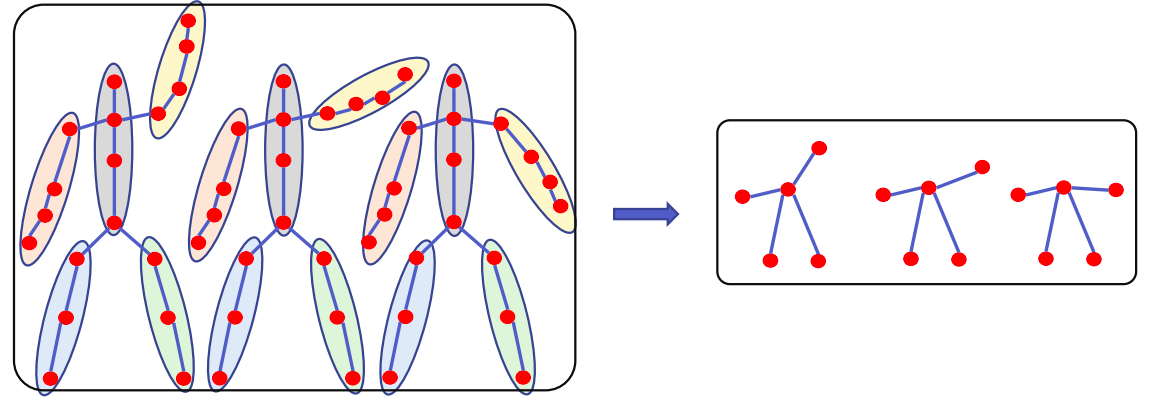
\includegraphics[width=\linewidth]{asset/image/body_part_embedding.png}
        \caption{Human body part embedding}
        \label{fig:body-part-embedding}
    \end{center}
\end{figure}